\documentclass[conference]{IEEEtran}
\usepackage[english]{babel}
\usepackage{amsmath}
\usepackage{amsthm}
\usepackage{graphicx}
\usepackage[utf8]{inputenc}
\usepackage{multirow}

%%%%%%%% SUB-FIGURE PACKAGE
\usepackage{subcaption}

%%%%%%%% HYPERREF PACKAGE
\usepackage{hyperref}
\hypersetup{linkcolor=blue}
\hypersetup{citecolor=blue}
\hypersetup{urlcolor=blue}
\hypersetup{colorlinks=true}

%%%%%%%% DEFINITION AND THEOREM DEFINITIONS
\theoremstyle{definition}
\newtheorem{definition}{Definition}[section]

\theoremstyle{remark}
\newtheorem{remark}{Remark}

\theoremstyle{remark}
\newtheorem{question}{Question}

\newtheorem{theorem}{Theorem}[section]

%%%%%%%% MULTI-COLUMNS PACKAGE
\usepackage{multicol}

%%%%%%%% BIB-LATEX STUFF
\usepackage[style=ieee,
            bibstyle=ieee,
            citestyle=ieee,
            hyperref=true,
            backend=biber]{biblatex}
\addbibresource{ref.bib} %Put relative path to ref

%%%%%%%% PERSONAL COMMANDS
\usepackage{amssymb}

%%%% Important sets
\renewcommand{\O}{\mathbb{O}}
\newcommand{\N}{\mathbb{N}}
\newcommand{\Z}{{\mathbb{Z}}}
\newcommand{\Q}{{\mathbb{Q}}}
\newcommand{\R}{{\mathbb{R}}}

%%%% Usual operations
\newcommand{\pow}[2]{#1^{#2}}
\newcommand{\expp}[1]{e^{#1}}
\newcommand{\fst}{\mathrm{fst}}
\newcommand{\snd}{\mathrm{snd}}

%%%% Lambda Calculus
\newcommand{\dneq}{\,\, \# \,\,}
\renewcommand{\S}{\pmb{\mathrm{S}}}
\newcommand{\I}{\pmb{\mathrm{I}}}
\newcommand{\K}{\pmb{\mathrm{K}}}
\newcommand{\ch}[1]{\ulcorner #1 \urcorner}

%%%% Ordinal Lambda Calculus
\newcommand{\ordAlph}{\Sigma_{\text{Ord}}}
\newcommand{\termOrd}{\text{Term}_\text{Ord}}
\newcommand{\fl}{\mathrm{fl}}
\newcommand{\sk}{\mathrm{sk}}

%% Superscript to the left
% https://latex.org/forum/viewtopic.php?t=455
\usepackage{tensor}
\newcommand{\app}[3]{\tensor*[^{#1}]{\left(#2, #3\right)}{}}

%%%% Make optional parameter
% https://tex.stackexchange.com/questions/217757/special-behavior-if-optional-argument-is-not-passed
\usepackage{xparse}

%%%% Statistics
\NewDocumentCommand{\E}{o m}{
  \IfNoValueTF{#1}
  {\mathbb{E}\left[#2\right]}
  {\mathbb{E}^{#1}\left[ #2\right]}
}
\NewDocumentCommand{\V}{o m}{
  \IfNoValueTF{#1}
  {\mathrm{Var}\left[#2\right]}
  {\mathrm{Var}^{#1}\left[ #2\right]}
}
\RenewDocumentCommand{\P}{o o m}{
  \IfNoValueTF{#1}
  {\IfNoValueTF{#2}
    {\mathrm{P}\left(#3\right)}
    {\mathrm{P}^{#2}\left(#3\right)}}
  {\IfNoValueTF{#2}
    {\mathrm{P}_{#1}\left(#3\right)}
    {\mathrm{P}_{#1}^{#2} \left(#3\right)}}
}

%%%% Lambda Calculus
\NewDocumentCommand{\cx}{o}{
  \IfNoValueTF{#1}
  {\left[\quad\right]}
  {\left[\, #1 \,\right]}
}

%%%% Create absolute value function
% https://tex.stackexchange.com/questions/43008/absolute-value-symbols
\usepackage{mathtools}
\DeclarePairedDelimiter\abs{\lvert}{\rvert}%
\DeclarePairedDelimiter\norm{\lVert}{\rVert}%
\makeatletter
\let\oldabs\abs
\def\abs{\@ifstar{\oldabs}{\oldabs*}}
%
\let\oldnorm\norm
\def\norm{\@ifstar{\oldnorm}{\oldnorm*}}
\makeatother

%%%%%%%% LOGIC TREES
\usepackage{prftree}

%%%%%%%% SPLIT EQUATIONS
% https://tex.stackexchange.com/questions/51682/is-it-possible-to-pagebreak-aligned-equations
\allowdisplaybreaks

%%%%%%%% FLOAT SPECIFIER
% https://www.overleaf.com/learn/latex/Errors/LaTeX_Error:_Unknown_float_option_%60H%27
\usepackage{float}

%%%%%%%% TO USE SHORT COMMANDS FOR VECTOR LINES
\usepackage{esvect}

%%%%%%%% ENUMERATE LABEL
% https://www.latex-tutorial.com/tutorials/lists/
\usepackage{enumitem}

%%%%%%%% DIFFERENT FONTS FOR MATH
\usepackage{mathrsfs}


\begin{document}

%%%%%% TITLE HEAD
\title{Unsupervised Learning Work}


\author{\IEEEauthorblockN{Juan Sebastián Cárdenas-Rodríguez}
  \IEEEauthorblockA{\textit{Department of Mathematical Science}\\
    \textit{Universidad EAFIT} \\
    Medellín, Colombia \\
    jscardenar@eafit.edu.co}}

\maketitle

\begin{abstract}
  In this work, an analysis of some unsupervised learning methods is tested in
  order to fully understand the inner work of the algorithms. Furthermore,
  optimal number of clusters and classification of the iris data set and a
  personal recollected data set is done. Finally, the source code for this work
  is given with all the algorithms and experiments.
\end{abstract}



\section{Introduction}
Mental health is crucially important for every human being and has become one of
the most important issues surrounding human health. According to the World
Health Organization\footnote{WHO's \href{https://bit.ly/34l2v94}{2001 report.}}
report of 2001, mental disorders can affect 25\% of the population, therefore,
suggesting the ongoing trend of people suffering from lack of mental health.

Furthermore, mental health is more important to monitor in adolescents and kids
as this group is in the process of developing their mental structure and
character. In this manner, as they continue creating their view about the world
they must be surrounded by a healthy environment that promotes healthy habits
and relationships with their surroundings.

As a result, schools and parents have an important responsibility to the
students of creating this environment and wisely handling mental health issues.
However, high schools do not always know how to handle or detect cases of mental
health issues. Additionally, technology has led to targeted harassing becoming
more popular over time, therefore, difficulting the probability of detecting
these cases.

Some of the most common and important mental health issues are anxiety,
depression, and hyperkinetic disorder. According to \textcite{schulte2016}, around
10\% to 20\% of children suffer from hyperkinetic disorder. Additionally, school
teachers just assume this disorder is a cause of undisciplined students and can
take the hyperkinetic student to a depressive state. These three mental
disorders can leave severe damage to a kid and can lead them to suicide.

Hence, it is of the utmost importance to quickly and efficiently detect students
that might be having a mental health issue to immediately start a process with
him/her. Furthermore, this detection has to be done with measurable variables
that can be easily obtained from questionnaires or school data.

Therefore, in this work an evaluation of the Psychological Attention Detection
(PAD) data set recollected with the help of the teacher will be classified and
evaluated. Furthermore, a testing data set will be used to first verify the
procedure done.


\section{Method} \label{sec:method}

There will be used 5 different clustering algorithms, for which 2 of them are
exploratory and 3 of them have a fixed number of clusters and find the best
classification given that number.

For the exploratory algorithms, the mountain clustering algorithm created by
\cite{yager1994} and the substractive clustering algorithm done by
\cite{chiu1994} will be used. It is acknowledge that both of this algorithms are
equivalent and only change the initial candidates for the prototypes.

On the other hand, for the fixed number of clusters the renown K-means algorithm
will be used. Furthermore, the Fuzzy C-means algorithm and the unnormalized
Laplacian spectral clustering presented by \cite{von2007} will be used. This are
mainly used in the real data set to verify how much does the clustering improve
when found the number of clusters.

\subsection{Clustering Validation}

For the cluster validation, two different inter-cluster indexes will be used. In
the first place, the \cite{calinski1974} index will be used. This a commonly
used inter-cluster index. Let $n$ be the number of data points, $K$, the number
of clusters, $C_{i}$ a set that contains the point of each cluster $i$,
$n_{i} = \abs{C_{i}}$ and $c_{i}$ the prototype for each cluster. The equation
for this index is given by:

\begin{equation*}
  \mathrm{CH} = \frac{n - K}{K - 1} \cdot
  \frac{\displaystyle\sum_{i=1}^{K} n_i \norm{c_i - \mu}^2}
  {\displaystyle\sum_{i=1}^K \sum_{x \in C_i} \norm{x - c_i}^2}
\end{equation*}

The idea for this measurement is to maximize this index in order to find a
better classification.

On the second hand, the inter-index done by \cite{davies1979} will be used. The
equation, using the same notation as the one above, for this index is given by:

\begin{align*}
  \mathrm{DB}
  &= \frac{1}{K} \sum_{i=1}^{K} \max_{j\neq i}\left\{\frac{\mu_{i} + \mu_{j}}
    {\norm{c_{i} - c_{j}}}\right\} \text{ where } \\
  \mu_{i} &= \frac{1}{n_{i}} \sum_{x \in C_{i}} \norm{x - c_{i}}
\end{align*}

Lastly, for the testing data set an extra-cluster index will be measured in
order to see if the classification is valid. Although this construction was done
empirically by the author, the idea to calculate the badly classified data
points. For this, one would classify good classification if a point belongs to a
cluster where the majority of the points have the same tag. Therefore, the
extra-cluster index is given by the number of badly classified points. It is
clearly seen that the idea is to minimize this value to obtain a better
classification.

The parameters chosen for each of the algorithms executed, are explicitly shown
on the source code as this article will focus mainly on the data analysis. The
source code was tested with \texttt{julia} 1.5.1 and it is given in an
\texttt{IJulia} notebook.

\section{Testing Data Set}

This section will cover the learnings and experiments done with the iris data
set in order to then apply the same principles in the real data set and explain
my reasoning in a smaller scale. Furthermore, in this section the higher
dimensions will not be covered as it is not essential for this testing data set.

In the first place, an exploration on the parameters for the substractive
clustering was realized in order to minimize the DH index and therefore find a
correct value for the parameters to find an optimal number of clusters. In
Figures \ref{fig:exp3d}, \ref{fig:exp3dman} and \ref{fig:exp3dmah} each of the
explorations with different norms can be found.

\begin{figure}[t]
  \centering
  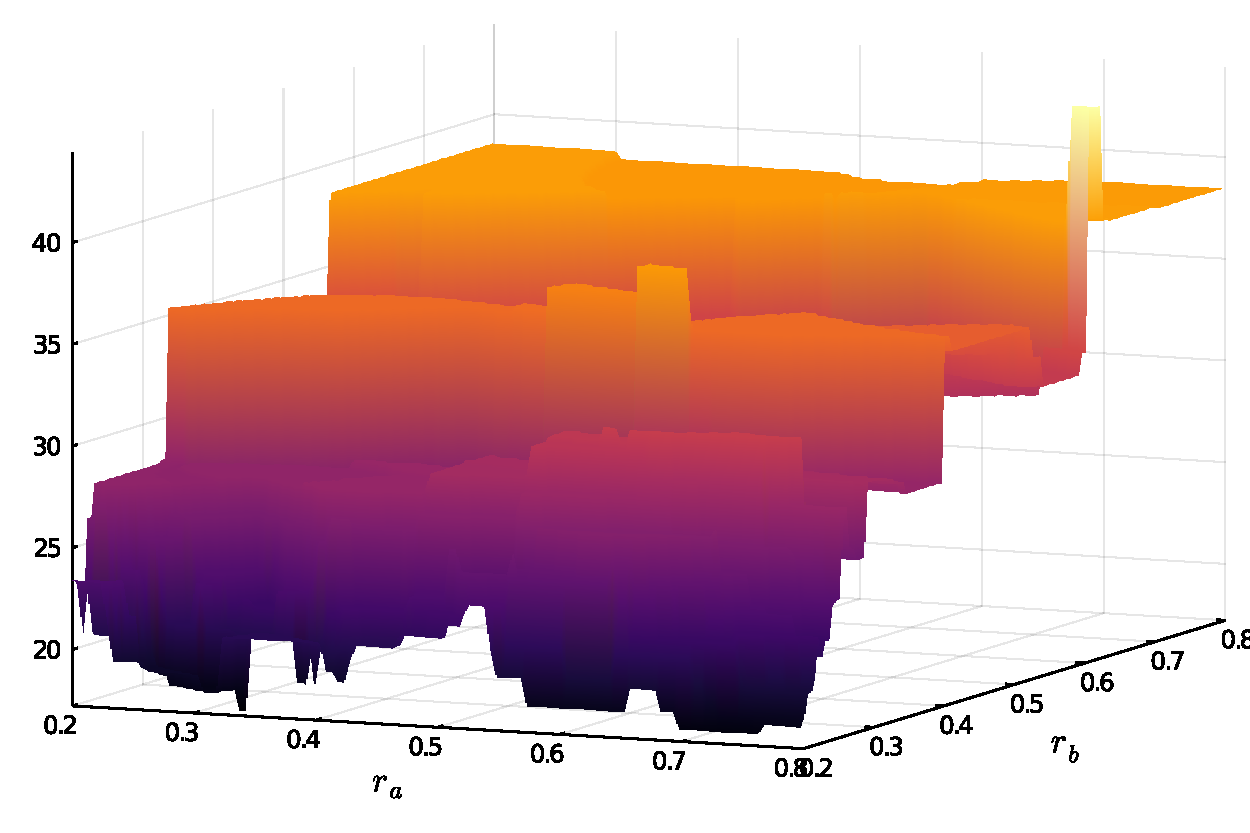
\includegraphics[scale=.35]{figs/iris/exploring-3d}
  \caption{Parameters $r_{a}$ and $r_{b}$ compared to DB index, with euclidean
    norm.}
  \label{fig:exp3d}
\end{figure}

\begin{figure}[t]
  \centering
  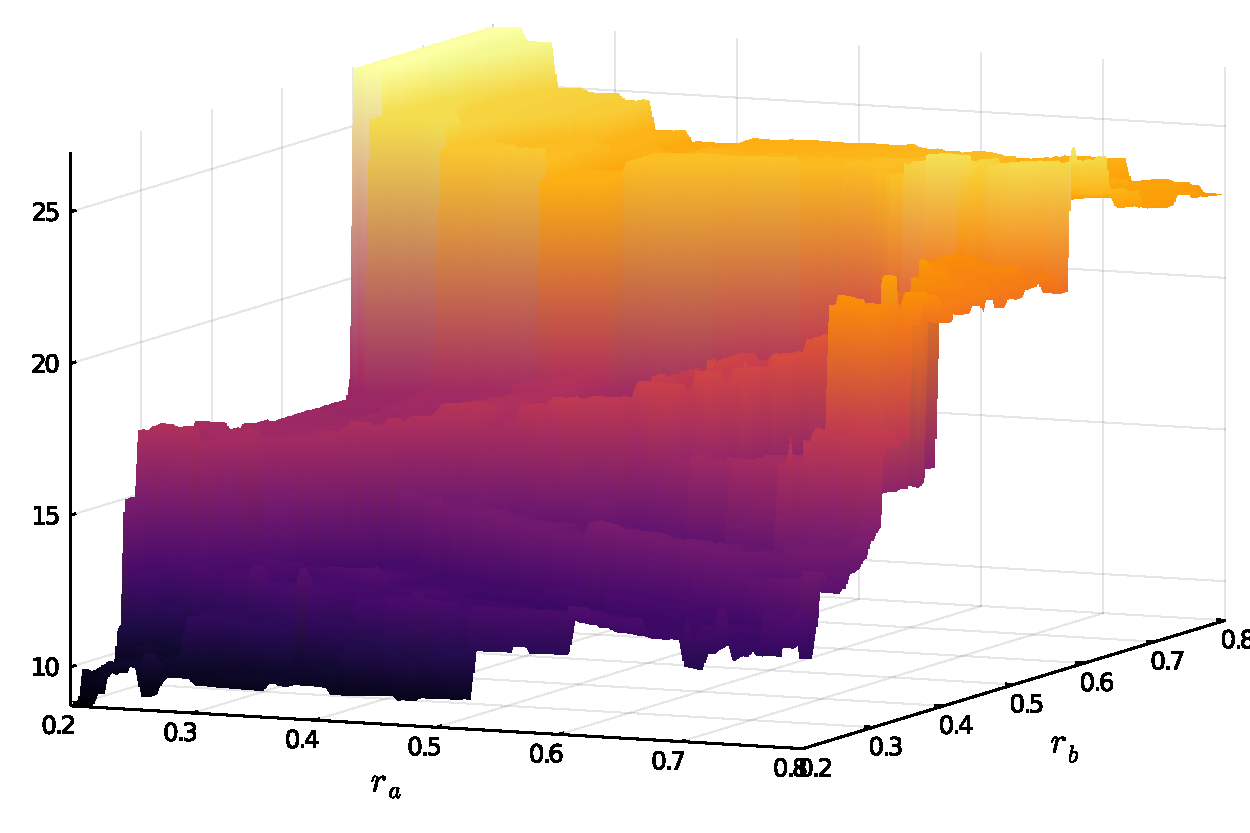
\includegraphics[scale=.35]{figs/iris/exploring-3d-man}
  \caption{parameters $r_{a}$ and $r_{b}$ compared to db index, with manhattan
    norm.}
  \label{fig:exp3dman}
\end{figure}

\begin{figure}[t]
  \centering
  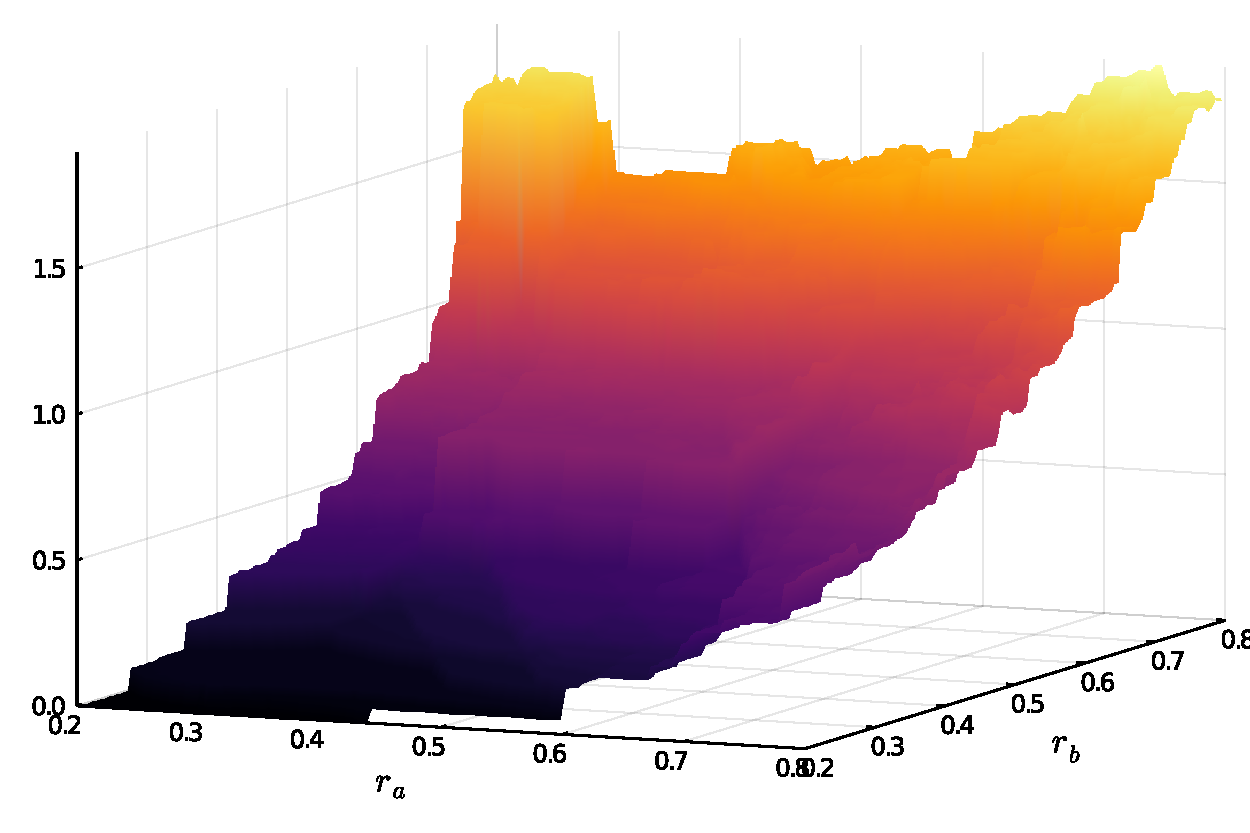
\includegraphics[scale=.35]{figs/iris/exploring-3d-mah}
  \caption{parameters $r_{a}$ and $r_{b}$ compared to db index, with mahalanobis
    norm.}
  \label{fig:exp3dmah}
\end{figure}

With this set of tests, it is clear that lower values of the parameter $r_{b}$
allow for a better classification as the DH index is lower. On the other hand,
in the author's work there is not a clear option to select from each of the
norms as they are almost the same. In this manner, a clear selection can not be
realized. The embedded iris data set will be used to further explain how to
choose the norm and each of the approach realized.

\subsection{Embedded Iris Data Set}

The iris data set was embedded to a 2D data set to simplify analysis and
visualization. It is important to remark that each time the embedding is
realized the data set is changed. Therefore, the results for this section will
be using one of the results obtained. The embedded data set can be seen in
Figure \ref{fig:embdata}.

\begin{figure}[t]
  \centering
  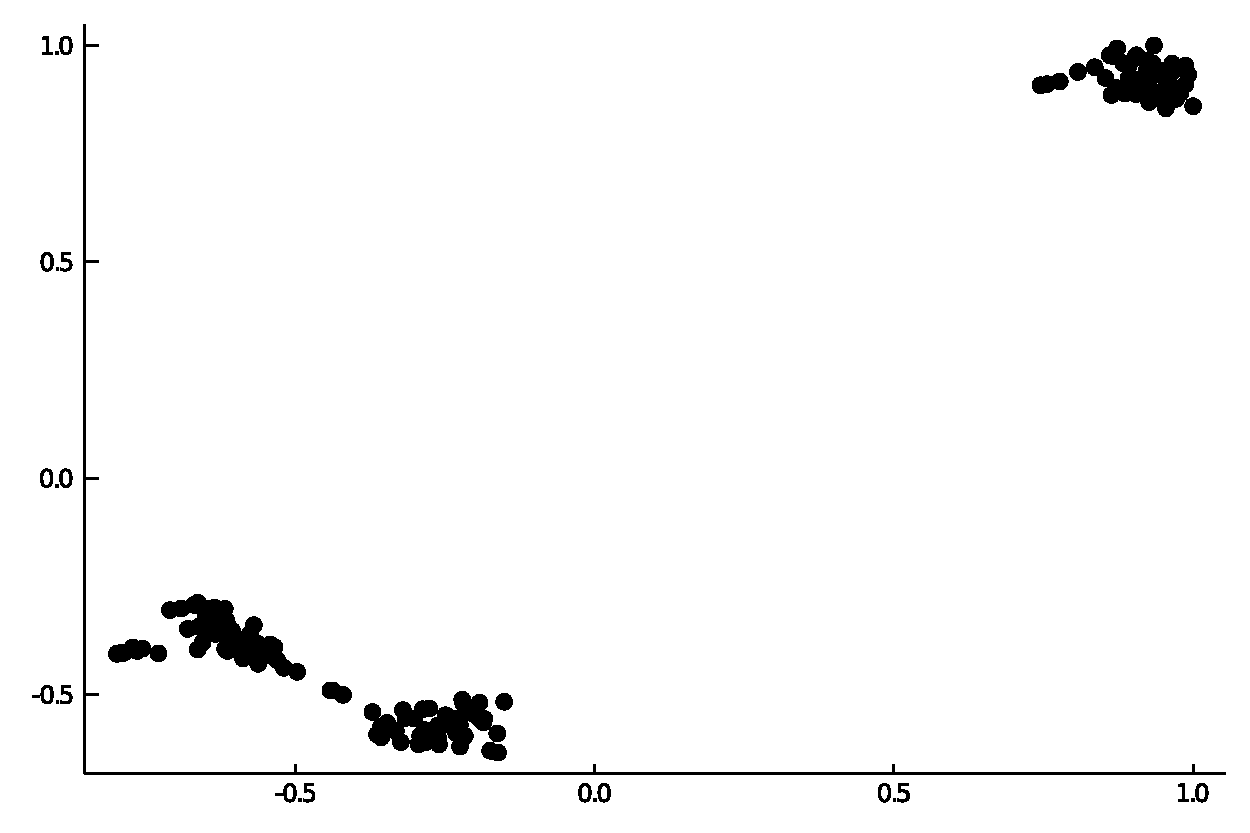
\includegraphics[scale=.35]{figs/iris/embedded-data-set}
  \caption{Embedded iris data set.}
  \label{fig:embdata}
\end{figure}

In the first place, the substractive clustering method was evaluated for
different values of parameters in order to understand how varying the parameters
affect the DH index. This would allow to have an understanding on what range of
parameters should be evaluated to test for an optimal number of clusters. In
Figure \ref{fig:expemb3d} the result of the DH index for the classification
given by the substractive clustering method for parameters $r_{a}$ and $r_{b}$
are shown using the euclidean norm.

\begin{figure}[t]
  \centering
  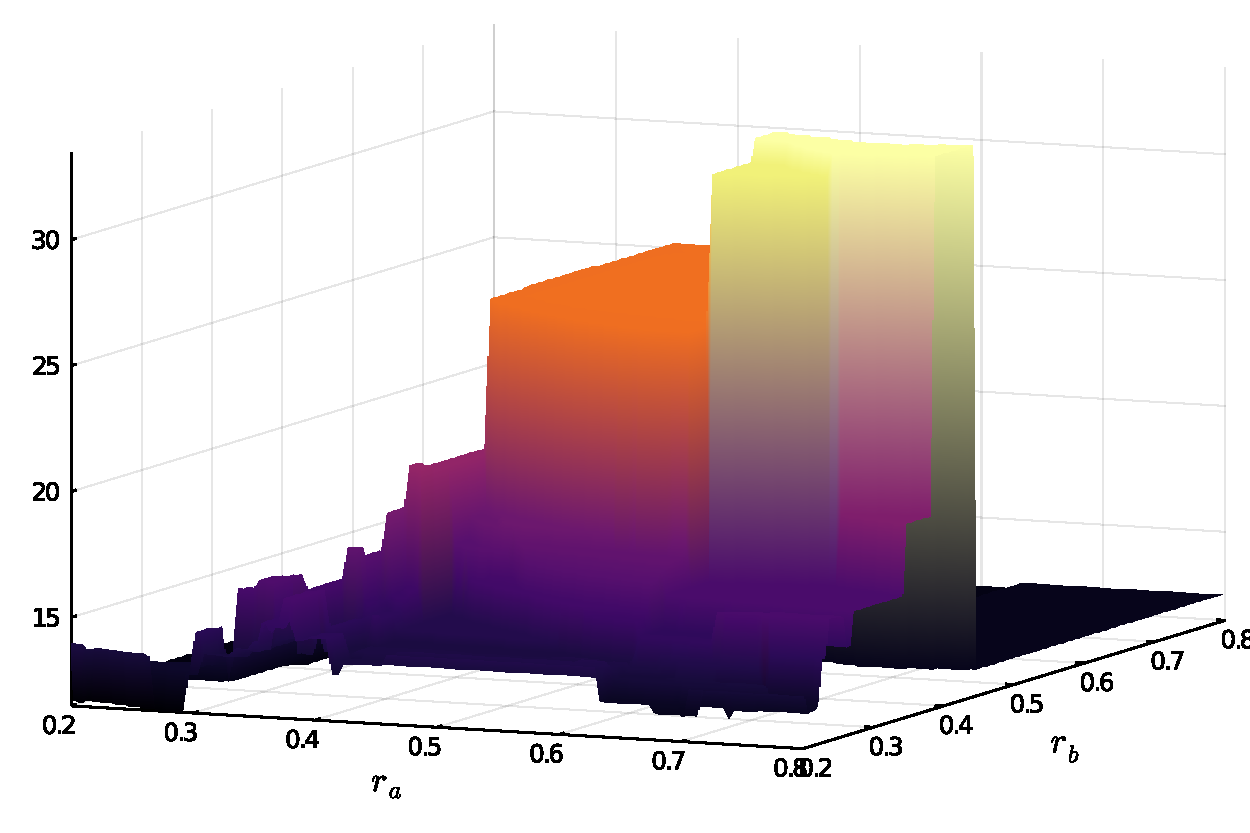
\includegraphics[scale=.35]{figs/iris/exploring-3d-emb}
  \caption{Parameters $r_{a}$ and $r_{b}$ compared to DB index, with euclidean
    norm.}
  \label{fig:expemb3d}
\end{figure}

In this manner, it is seen that for lower values of the parameter a better
result for the DH index is obtained. Furthermore, to confirm that the euclidean
norm did not biased the results also the manhattan and mahalanobis norm were
tested. In Figures \ref{fig:expemb3dman} and \ref{fig:expemb3dmah} the results
of each norm can be found.

\begin{figure}[t]
  \centering
  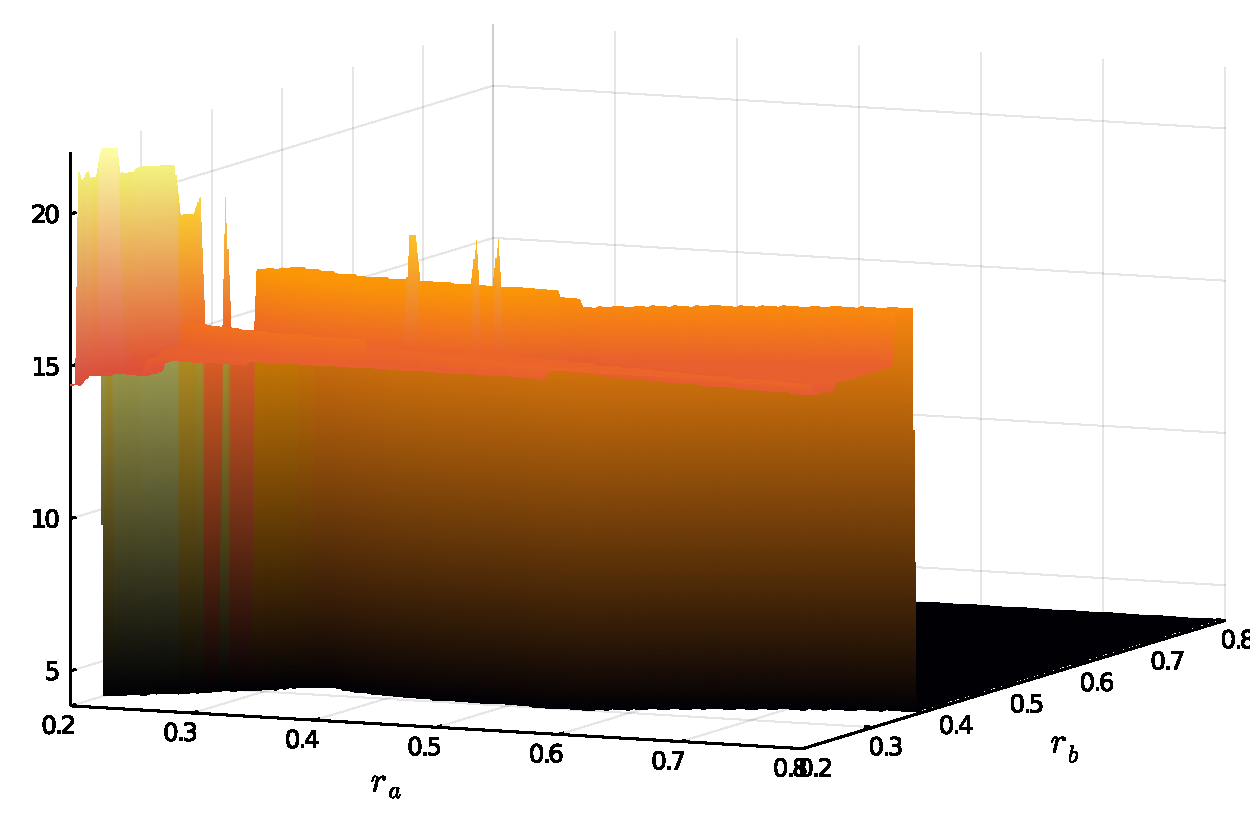
\includegraphics[scale=.35]{figs/iris/exploring-3d-emb-man}
  \caption{Parameters $r_{a}$ and $r_{b}$ compared to db index, with manhattan
    norm for embedded iris data set.}
  \label{fig:expemb3dman}
\end{figure}

\begin{figure}[t]
  \centering
  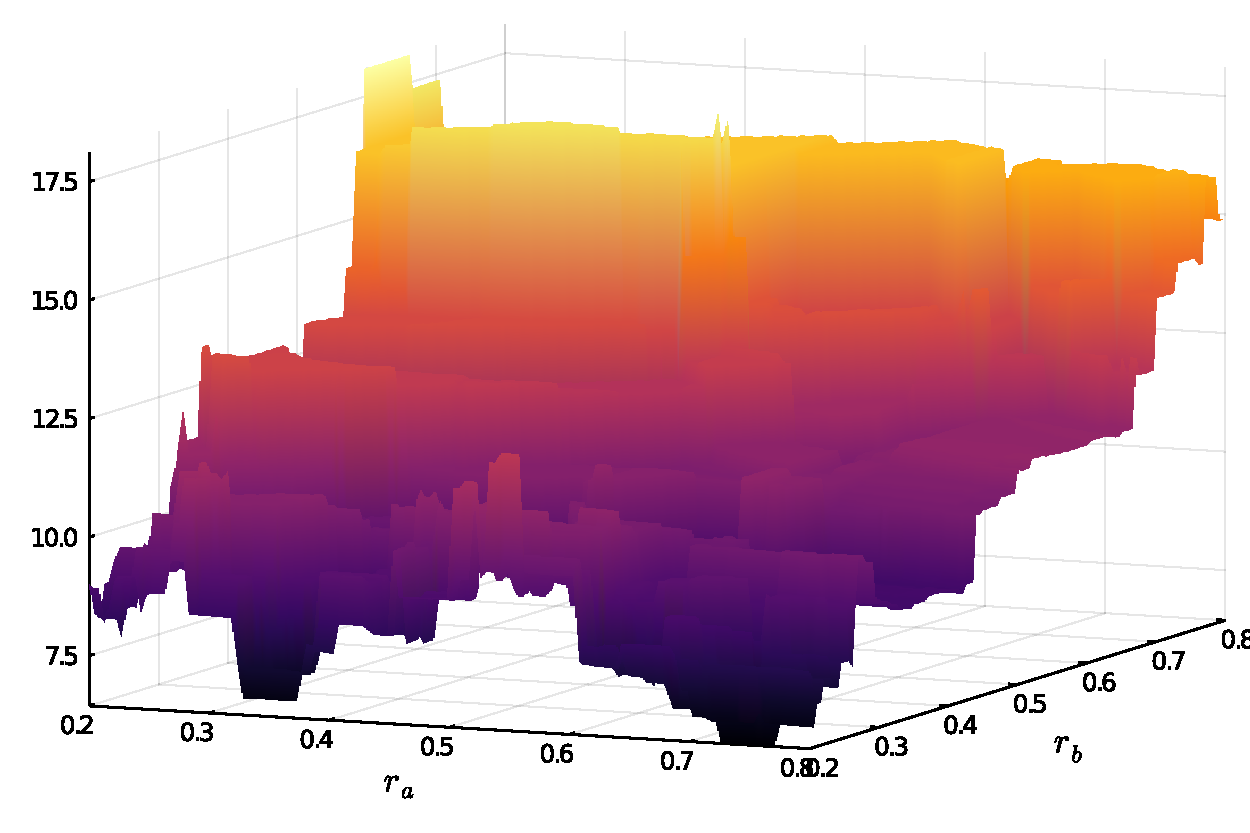
\includegraphics[scale=.35]{figs/iris/exploring-3d-emb-mah}
  \caption{Parameters $r_{a}$ and $r_{b}$ compared to db index, with mahalanobis
    norm for embedded iris data set.}
  \label{fig:expemb3dmah}
\end{figure}

The manhattan norm did confirmed that lower values of the parameter improve the
intra-cluster index. On the contrary it is seen that the for bigger values the
DH index suddenly converges to 0. This occurs because the method did not select
a second cluster, hence proving useless in clustering the data.

Using the mahalanobis norm much interpretation could not be obtained as there is
not an evident relationship between the parameters and the DH index. In this
manner, the euclidean norm will be used for the rest of this exercise as it
presents a clear trend and it is easy to run.

Accordingly to the analysis made, to test the mountain clustering method the
parameter $\sigma$ can be fixed in the interval $(0, 0.5)$ to obtain an optimal
result. Additionally, for simplicity, the other parameter was fixed at
$\beta = 1.5\sigma$. Therefore, in Figures \ref{fig:expembch},
\ref{fig:expembdb} and \ref{fig:expembn} the CH index, DB index and number of
clusters for different values of $\sigma$ can be found respectively.

\begin{figure}[t]
  \centering
  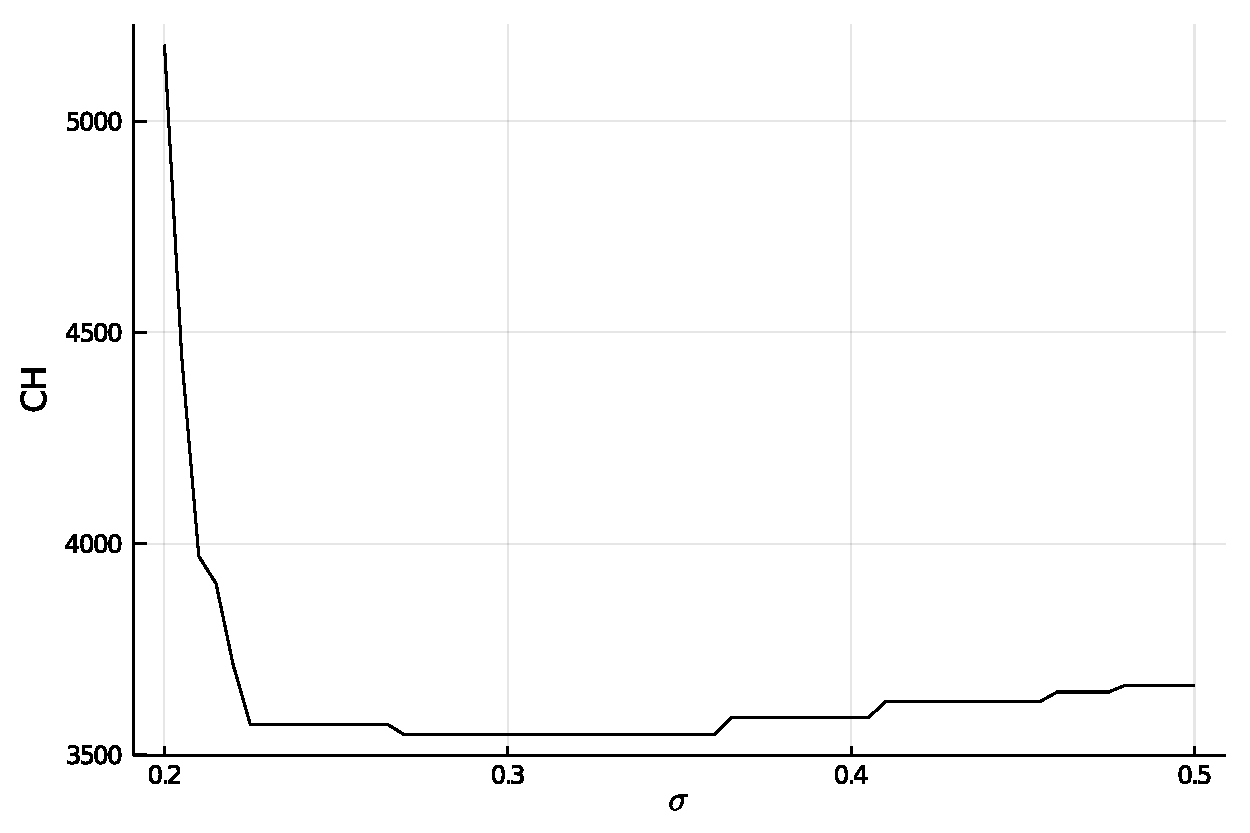
\includegraphics[scale=.35]{figs/iris/exploring-2d-emb-ch}
  \caption{CH index for embedded iris data set.}
  \label{fig:expembch}
\end{figure}

\begin{figure}[t]
  \centering
  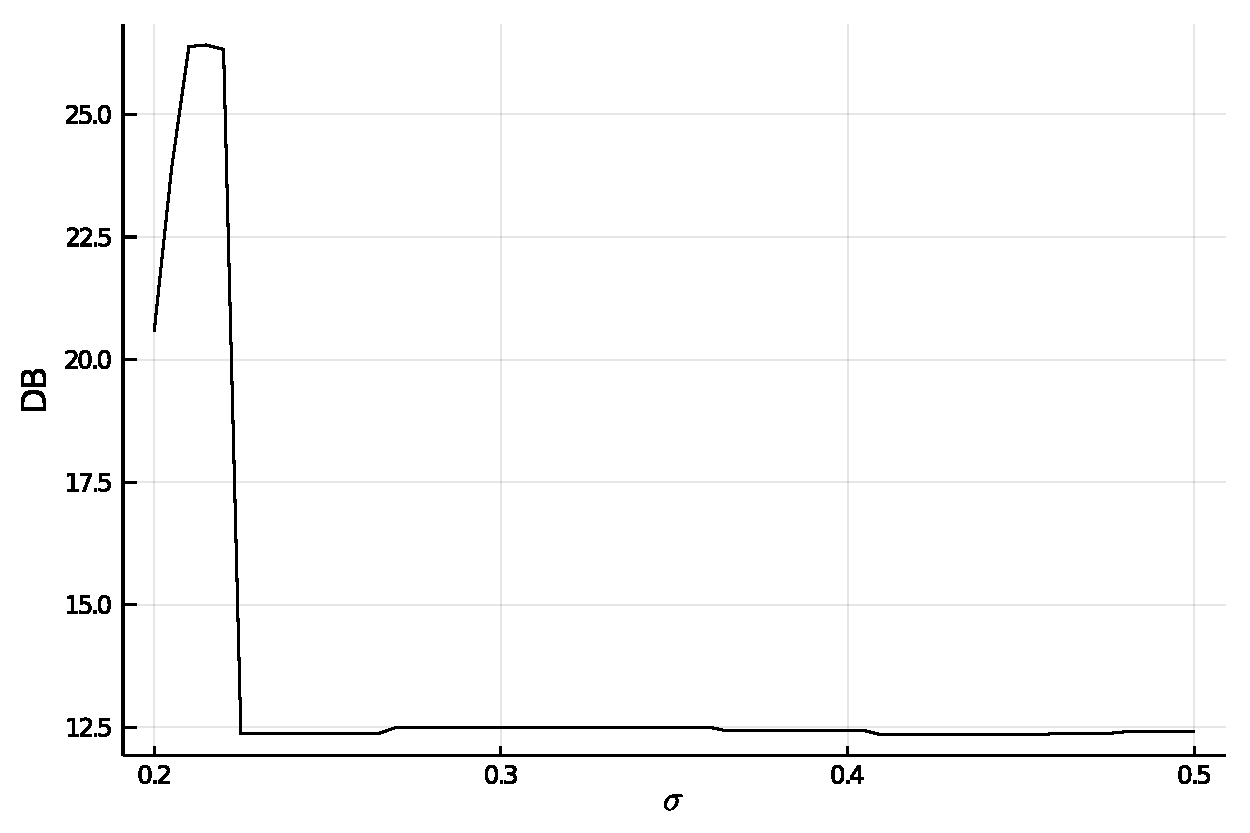
\includegraphics[scale=.35]{figs/iris/exploring-2d-emb-db}
  \caption{DB index for embedded iris data set.}
  \label{fig:expembdb}
\end{figure}

\begin{figure}[t]
  \centering
  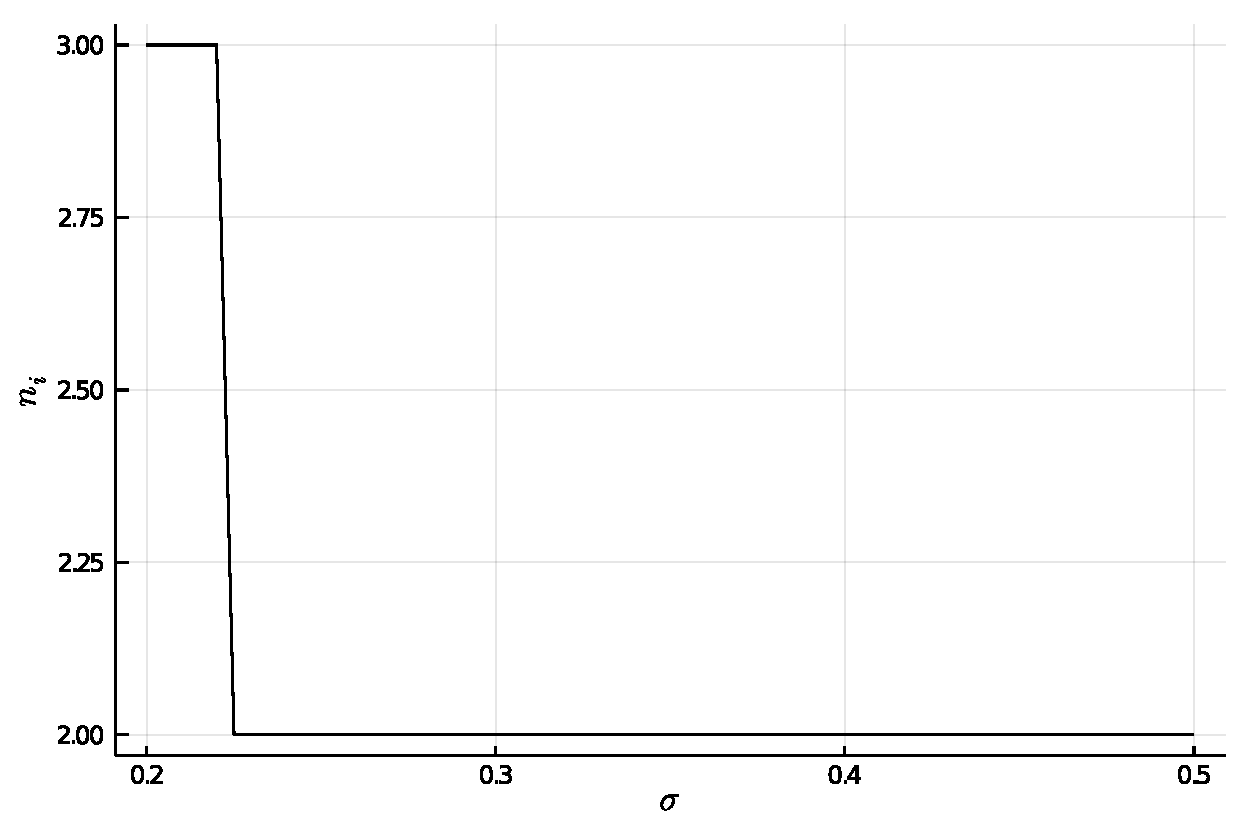
\includegraphics[scale=.35]{figs/iris/exploring-2d-emb-n}
  \caption{Number of clusters for embedded iris data set.}
  \label{fig:expembn}
\end{figure}

The goal, following the ideas of Section \ref{sec:method}, is to maximize the CH
index and minimize the DB index. In this manner, it is concluded with this
exploratory analysis that the best number of clusters would be to use 3 as it
satisfies the criterion explained. Furthermore, it is seen that the best
prototypes obtained by this method was given by the initial parameter tested
$\sigma=0.2$.

Furthermore, this is confirmed also by an extra cluster analysis, as the iris
data set has three different labels i.e. the data is clustered into 3 groups.
Therefore, it is important to notice that an exploratory analysis of the
clusters allows to find a good set of groups even if the ``real data'' is not
known.

Now with the fixed selected number of clusters, the three fixed clustering
methods can be used to obtain better clustering and prototypes. The results of
each of the three clustering methods can be seen in Figures \ref{fig:embk},
\ref{fig:embfc} and \ref{fig:embsc}.

\begin{figure}[t]
  \centering
  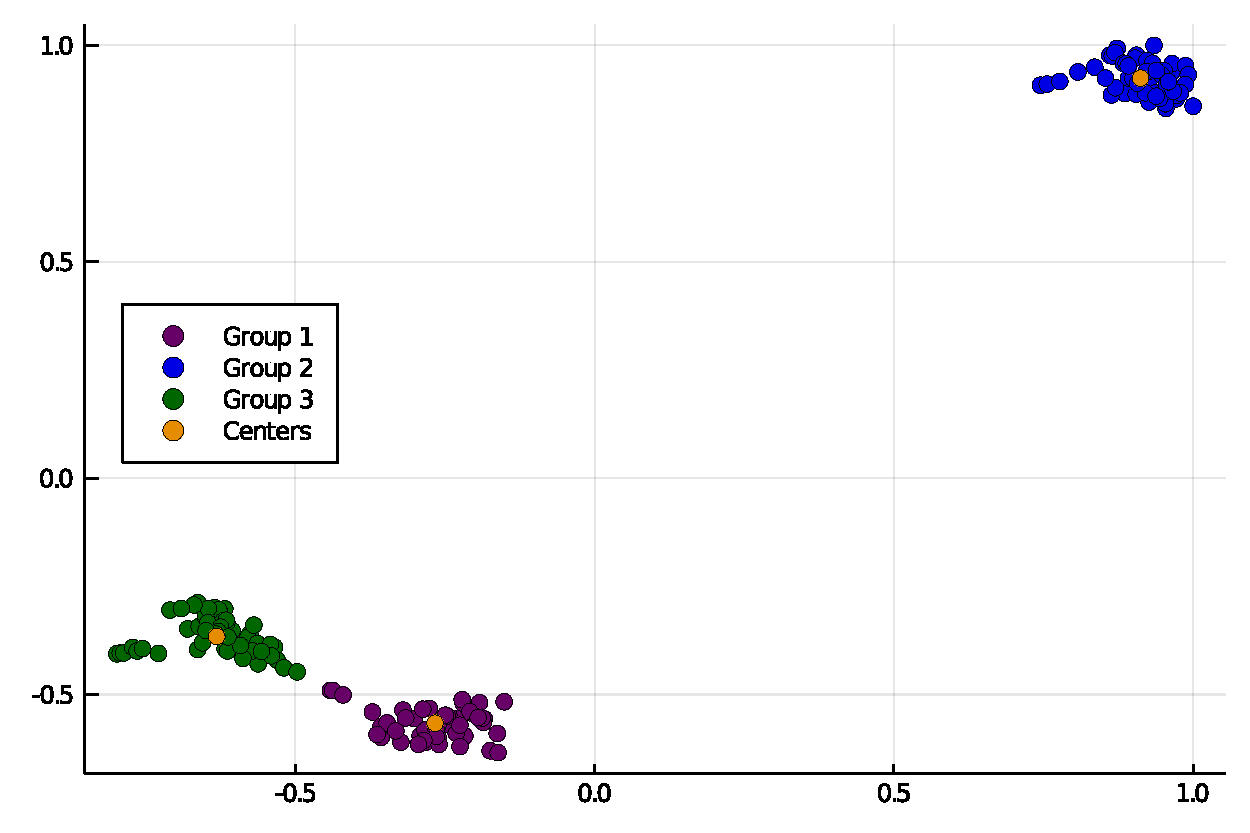
\includegraphics[scale=.35]{figs/iris/emb-k-means}
  \caption{K-means clustering for embedded iris data set.}
  \label{fig:embk}
\end{figure}

\begin{figure}[t]
  \centering
  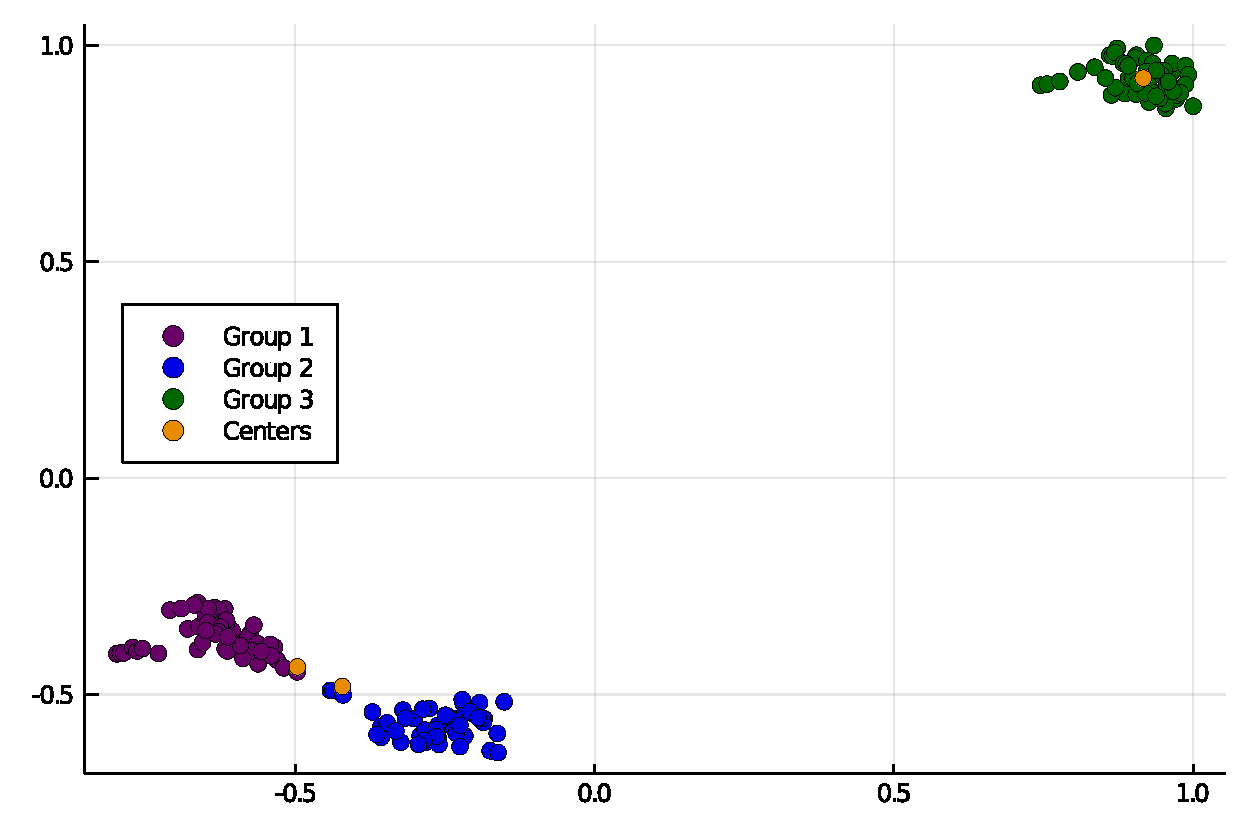
\includegraphics[scale=.35]{figs/iris/emb-fc-means}
  \caption{Fuzzy c-means clustering for embedded iris data set.}
  \label{fig:embfc}
\end{figure}

\begin{figure}[t]
  \centering
  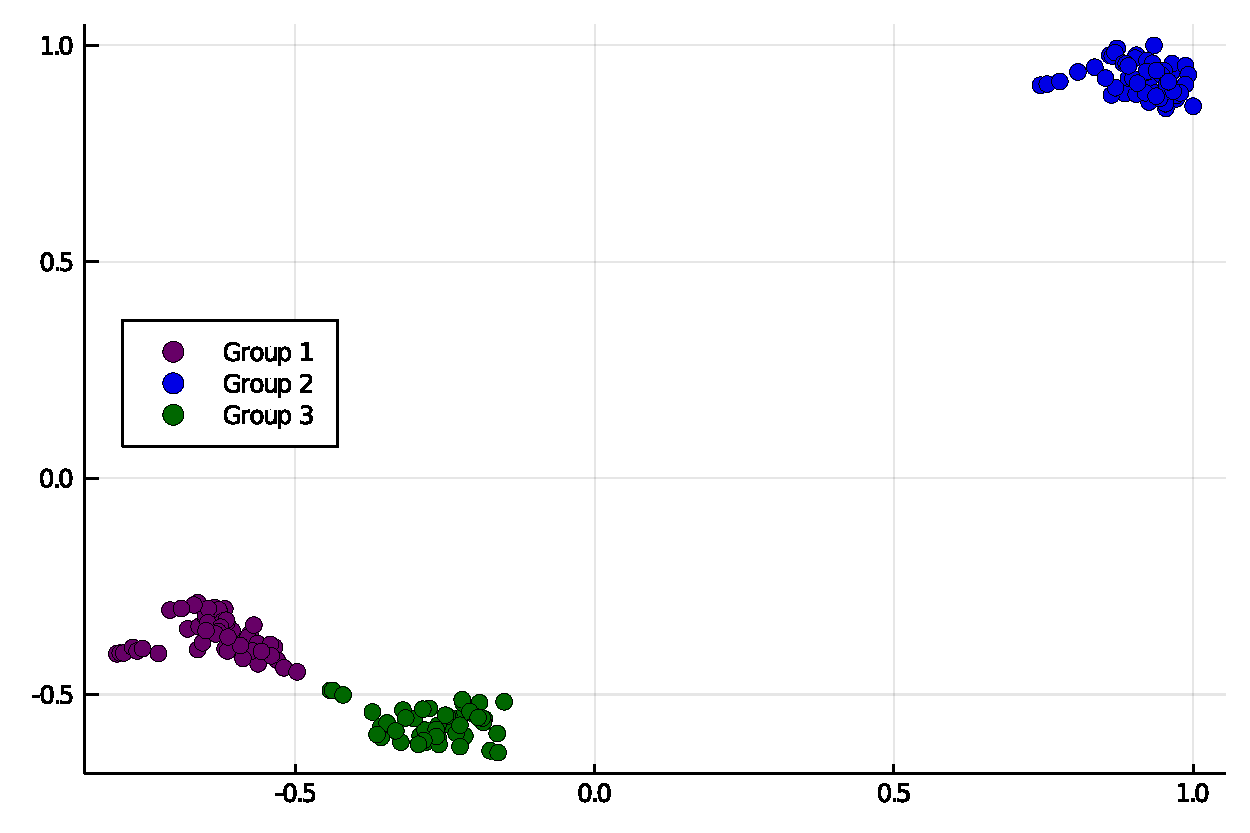
\includegraphics[scale=.35]{figs/iris/emb-spectral-clustering}
  \caption{Spectral clustering for embedded iris data set.}
  \label{fig:embsc}
\end{figure}

In the first place, it is noticed that the K-means algorithm successfully
partitioned the data as one would instinctively cluster it. The same can be said
surrounding the spectral clustering method. On the other hand, the fuzzy c-means
converged to some centers that do not seem according to the data set given.
Although some values for $m$ where tested and the same result was obtained, the
value for this parameter could be the cause of this convergence.

In the second place, to understand why would this algorithms be necessary
instead of using only the exploratory algorithms comparison between the
performance of the mountain clustering and the other algorithms is showed in
Table \ref{tab:compemb}.

\begin{table}
  \begin{tabular}{ccccc}
    \hline
    & Mountain & K-Means & Fuzzy C-Means & Spectral \\
    Ext. Index & 5       & 2         & 2            & 2                   \\
    DB Index   & 20.58   & 12.17     & 130.93       & N/A                 \\
    CH Index   & 5180.66 & 108011.97 & 2603.10      & N/A \\ \hline
  \end{tabular}
  \caption{Comparison between each of the methods.}
  \label{tab:compemb}
\end{table}

Without taking into account the fuzzy c-means algorithm, the fixed cluster
algorithms improved the intra-cluster and extra-cluster values in comparison
with the exploratory algorithm. This occurs because fixed cluster algorithms,
such as K-means, improve on an objective function instead of trying to explore
the space for a good clustering number. Hence, this method help the ``goodness''
of the clusters.

In conclusion, the embedded data set allowed to visualize the behavior of the
data without breaking their structure drastically. Furthermore, the clustering
algorithms where able to detect the optimal number of clusters and, almost,
completely characterize the data. Lastly, it allows for a quicker run of this
algorithms as it reduces the dimensions of the original data set.


\section{PAD Data Set}
In the first place, a preliminary analysis will be done with the embedded data
set to extract some information about the structure of the original data set as
the data set cannot be visualized. Furthermore, this analysis allows to have a
basic visualization on what it would be expected to have on higher dimensions.

\subsection{Embedded PAD Data Set}

In Figure \ref{fig:embds} the embedded data set can be seen. At first glance, it
is seen, intuitively, that this reduced data set posses two different marked
groups. In this manner, an exploratory analysis is deemed to not be necessary
for this special case. Therefore, just by visualizing, the fixed cluster
algorithms will be tested with 2 clusters. Furthermore, the norm was selected to
be the euclidean norm as the clusters are clearly circular.

\begin{figure}[t]
  \centering
  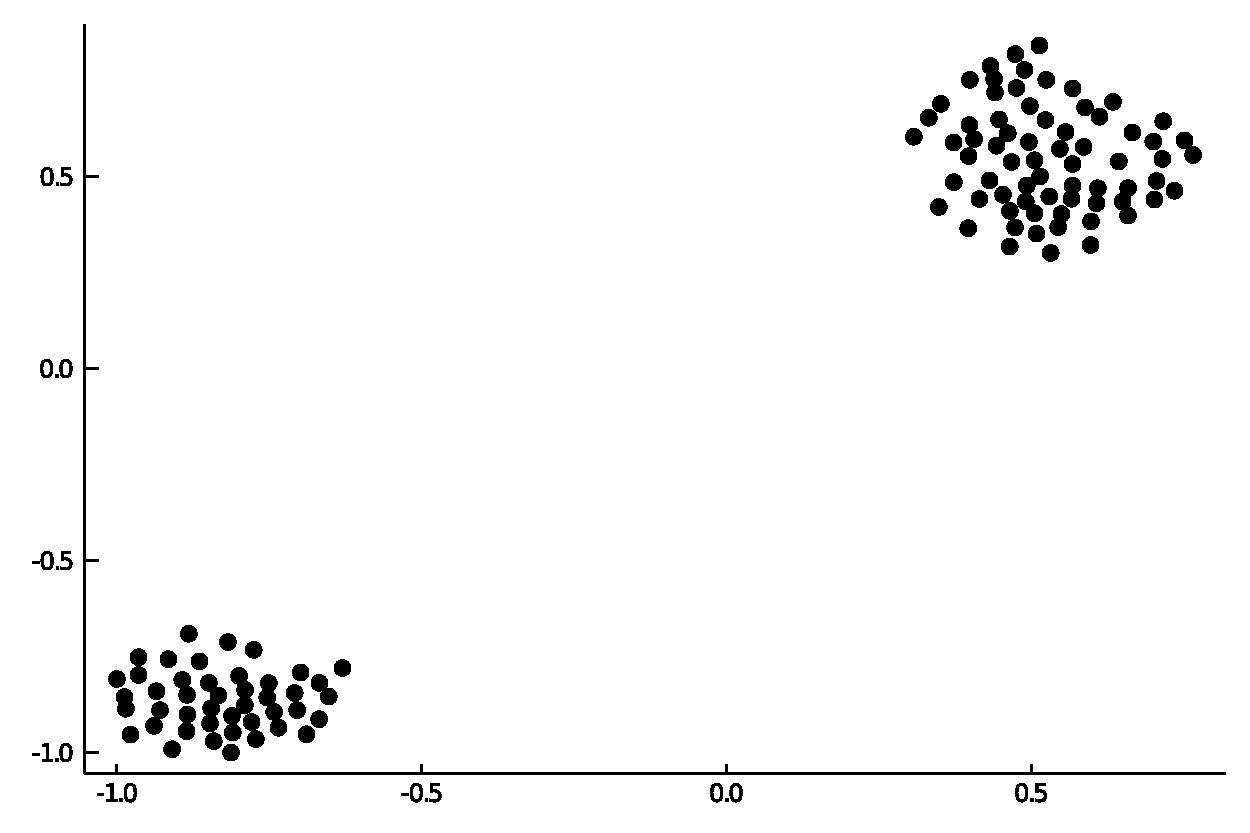
\includegraphics[scale=.3]{figs/real/embedded}
  \caption{Embedded data set.}
  \label{fig:embds}
\end{figure}

Consequently, in Figures \ref{fig:embdsk}, \ref{fig:embdsfc} and
\ref{fig:embdssc} the results for the chosen three fixed cluster algorithms can
be found. As it was expected, the results for each of the algorithms is perfect
as the separation between the groups is pretty significant. Each of the
algorithms converge quickly, confirming this statement.

On the other hand, as the separation is that marked, it is hard to actually find
a significant difference between the classification done by each of the methods.
Furthermore, as is not possible to check for external indexes this grouping it's
hard to verify.

\begin{figure}[t]
  \centering
  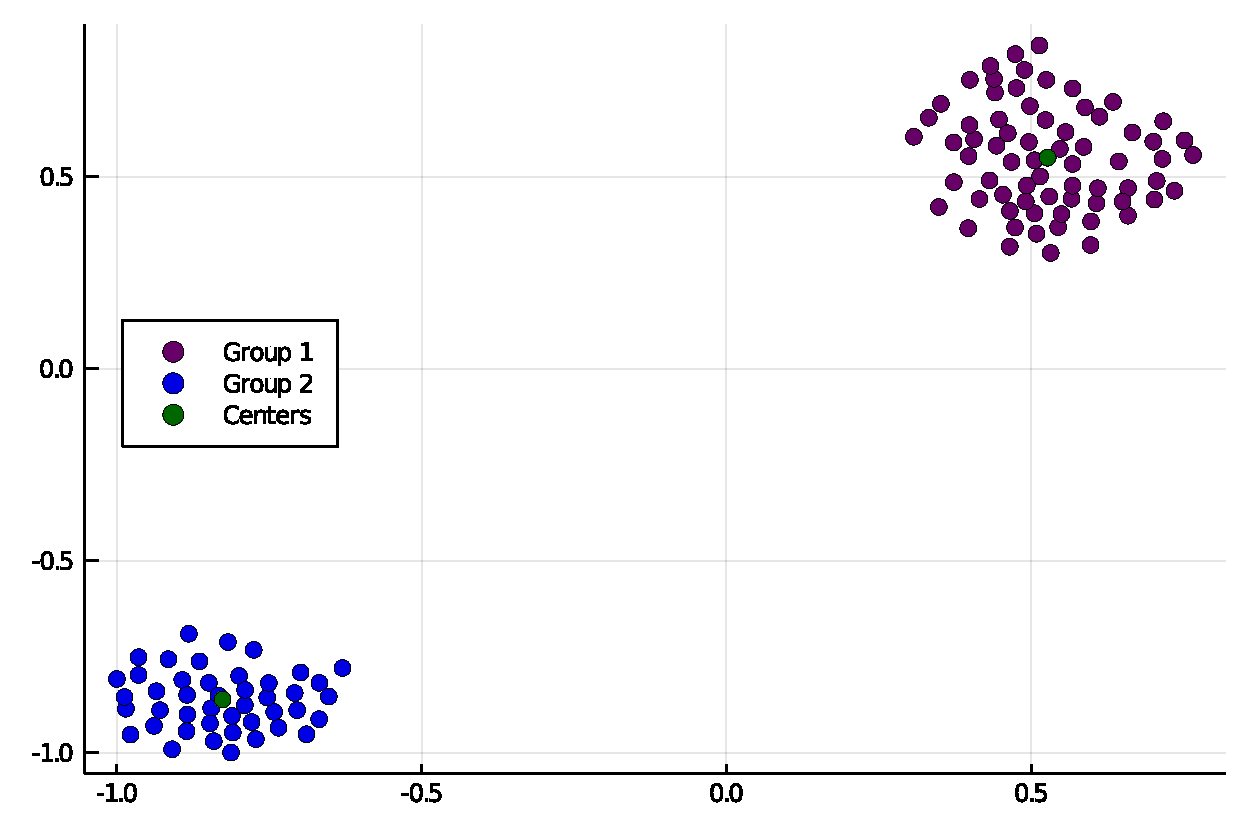
\includegraphics[scale=.35]{figs/real/emb-k-means}
  \caption{K-means clustering for embedded PAD data set.}
  \label{fig:embdsk}
\end{figure}

\begin{figure}[t]
  \centering
  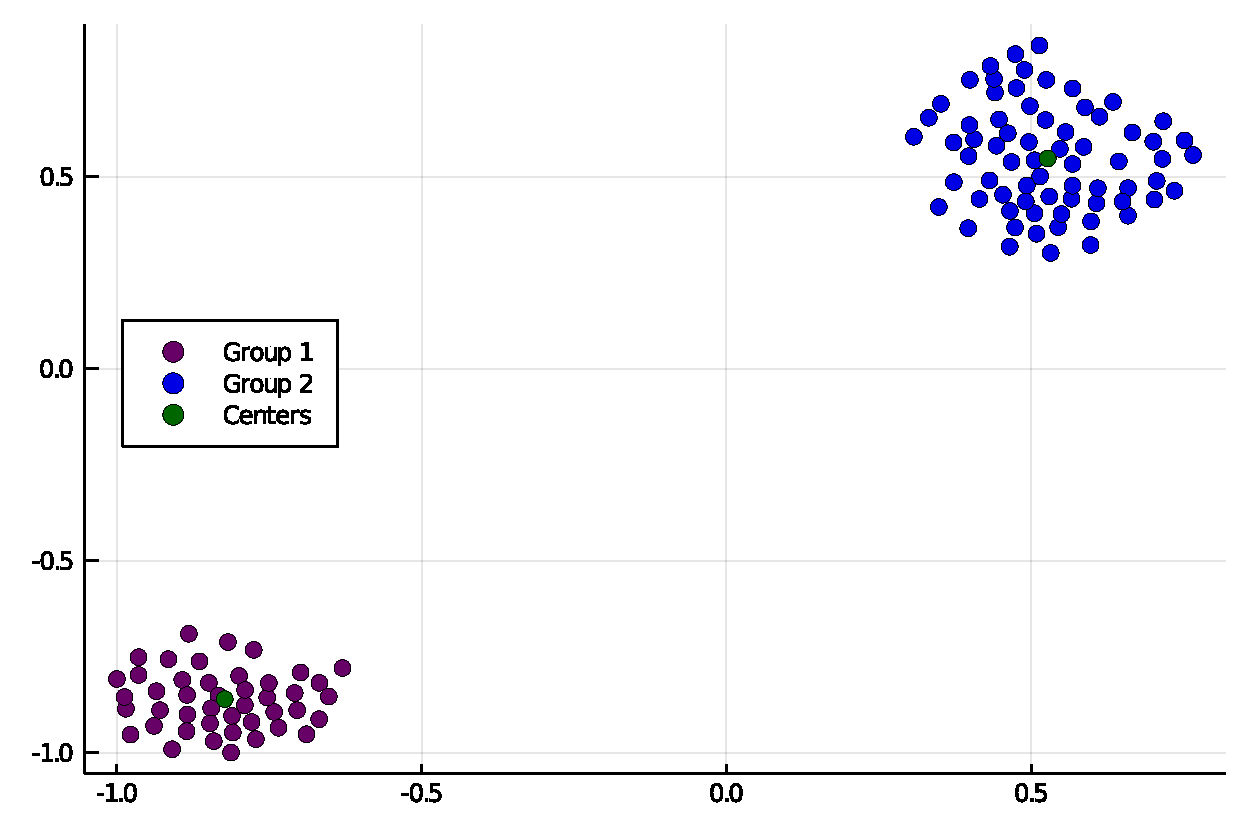
\includegraphics[scale=.35]{figs/real/emb-fc-means}
  \caption{Fuzzy c-means clustering for embedded PAD data set.}
  \label{fig:embdsfc}
\end{figure}

\begin{figure}[t]
  \centering
  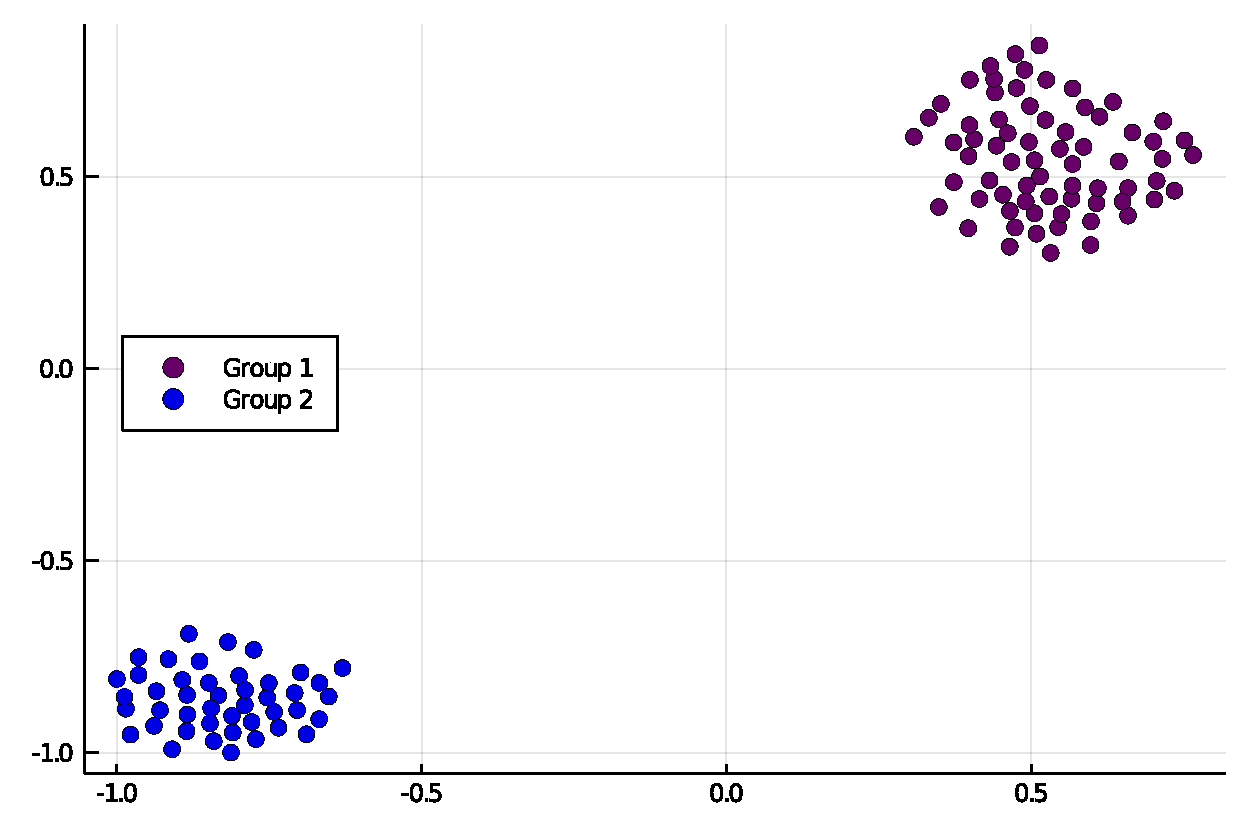
\includegraphics[scale=.35]{figs/real/emb-spectral-clustering}
  \caption{Spectral clustering for embedded PAD data set.}
  \label{fig:embdssc}
\end{figure}

On the other hand, the main goal for obtaining this data was to be able to
diagnose if a student should be receive psychological attention to bring them
early help before their situation goes out of control. In this manner, it is
curious that the embedded data separated so clearly between two groups on the
opposite vertex of the rectangle that encloses the data. It is important to
further analyze if this separation fulfills the desired role.

In conclusion, the embedding of the data presented a clear separation between
two groups that where easily separated. Furthermore, as the embedding preserves
topology for the data, the euclidean norm will be the norm used for the next
experiments although the number of clusters will still be tested with
exploration clustering algorithms.

\subsection{PAD Data Set}

Following the ideas explored in the testing data set, a table for the changes of
the DH index by changing the parameter of the substractive clustering algorithm
was realized in order to understand which set of parameters should be essential
to obtain a good number of clusters. For this experiment, the value for $r_{a}$
was changed while $r_{b}$ was fixed at $1.5r_{a}$. In this manner, in table
\ref{tab:expds} the results for this exploration can be found.

\begin{table}
  \centering
  \begin{tabular}{cccc}
    \hline
    $r_a$ & $n_i$ & DB    & CH     \\
    0.2   & 87    & 1.10  & 36.35  \\
    0.3   & 30    & 4.79  & 42.23  \\
    0.4   & 11    & 15.97 & 55.40  \\
    0.5   & 5     & 31.21 & 85.90  \\
    0.7   & 3     & 30.88 & 146.97 \\
    0.8   & 2     & 35.86 & 232.13 \\
    1.5   & 2     & 28.67 & 150.46 \\ \hline
  \end{tabular}
  \caption{Properties of clusters for different values of $r_{a}$}
  \label{tab:expds}
\end{table}

In the table, the values that are jumped with a bigger difference than 0.1 is
that it stayed constant for the evaluation. In this manner, it is seen that
there was an ``optimal'' found at $r_{a}=0.8$ as seen in how the CH index
changes. Furthermore, as it stays constant for a bit it makes sense that it
would actually be in a valley until changing again. Lastly, this value coincides
with the one obtained with the embedded data.

In this manner, at this moment the embedded data takes meaning in the manner
that, although it extremely simplified the data set, it allows to extract
characteristics that still may preserve in higher dimensions. Furthermore, this
is also verified by seen the obtained value for the inter cluster.

Analogously, let's find the values for the respective indexes when the fixed
clustering method is used. Furthermore, let's test this values for both 2 and 3
clusters in order to fully confirm the number of groups. In Table \ref{tab:clds}
the results for each of the methods for different number of clusters can be
found.

\begin{table}
  \centering
  \begin{tabular}{cccc}
    \hline
    \multicolumn{1}{l}{$n_i$} & Method   & DB     & CH     \\ \hline
    \multirow{2}{*}{2}        & K-means  & 42.00  & 174.55 \\
                              & FC-Means & 50.95  & 118.20 \\ \hline
    \multirow{2}{*}{3}        & K-means  & 36.13  & 131.14 \\
                              & FC-Means & 148.29 & 3.26   \\ \hline
  \end{tabular}
  \caption{Result for each of the clustering algorithms.}
\label{tab:clds}
\end{table}

In this manner, it is clearly seen that the optimal number of classifications
done is 2 as, specially, fuzzy c-means do not have a good behavior when trying
to separate the group onto three groups. Therefore, the obtained result for the
embedded data still continue to be valid in higher dimensions.

On the other hand, the spectral clustering can not be thoroughly tested as the
indexes for testing clusters need a center and spectral clustering does classify
by graph connections. Therefore, this method for this and the following
experiment will not be used.

In conclusion, as obtained with the embedded data, the optimal number of
clusters to classify the PAD data set is 2. This affirms how embedding data can
be useful to get preliminary information from the data, with an easy
visualization in processable information. Lastly, the different fixed clustering
methods help to decide the optimum value by evaluating the different
inter-cluster indexes.

\subsection{Higher Dimension PAD Data Set}

To increase the dimension of the PAD data set, two main characteristics were
extracted from the original data. In the first place, the moving average for
each of the data is calculated. Lastly, the discrete Fourier transform was
calculated for each of the data and the absolute value of each transform was
extracted to not use complex values. Hence, for each of this characteristics new
6 columns are generated hence tripling the dimensions of the original data set.

Following the ideas in the previous section, in Table \ref{tab:exphds} the
results of the indexes for different values of $r_{a}$ are shown. It is
important to remark that the mountain clustering algorithm is not used in this
section to avoid the grid creation that, usually is really computationally
heavy; furthermore, the substractive and mountain algorithm are basically the
same but with different candidates.

\begin{table}
  \centering
  \begin{tabular}{cccc}
    \hline
    $r_a$ & $n_i$ & DB    & CH    \\
    0.3   & 112   & 0.37  & 7.76  \\
    0.4   & 84    & 2.27  & 8.28  \\
    0.5   & 40    & 6.54  & 11.35 \\
    0.6   & 14    & 16.22 & 19.86 \\
    0.7   & 7     & 35.39 & 29.71 \\
    0.8   & 4     & 42.05 & 48.70 \\
    0.9   & 3     & 45.09 & 64.94 \\
    1.3   & 2     & 61.75 & 93.15 \\
    1.5   & 2     & 70.02 & 74.51 \\ \hline
  \end{tabular}
  \caption{Properties of clusters for different values of $r_{a}$}
  \label{tab:exphds}
\end{table}

Analogously, it is seen that a similar behavior than the normal data set is
found. As $r_{a}$ starts changing, in each iteration there is an improvement in
one of the indexes, therefore not giving an optimal solution. Finally, in
$r_{a}=1.3$ an optimal value as changing the parameter even further degenerates
both indexes without improving. In this manner, as expected, the number of
clusters given are still 2.

In conclusion, the higher data set allowed to extensively confirm the already
established hypothesis. In this manner, these three data spaces proven give us a
full view of the data set and fully inform us about it's behavior and
classification.

\section{Conclusion}

In conclusion, in the iris data set and the PAD data set it was shown the
usefulness of the clustering algorithms to correctly explain a data set.
Furthermore, it was seen that using different dimensions for the same data set
helps to grasp and confirm information of the data set, to find discrepancies
and to evaluate the structure of the data.

\printbibliography
\end{document}
